\documentclass[10pt, hyperref={hidelinks}]{beamer}

%\usepackage{algorithm}
%\usepackage[noend]{algpseudocode}
\usepackage{amsfonts}
\usepackage{amsmath}
\usepackage{amssymb}
\usepackage{amsthm}
\usepackage[ngerman]{babel}
\usepackage[backend=biber, citestyle=numeric-comp, bibstyle=ieee]{biblatex}
%\usepackage{changepage}
\usepackage{enumitem}
%\usepackage{fancyhdr}
%\usepackage{fontspec}
%\usepackage{fullpage}
\usepackage{mathtools}
\usepackage{physics}
\usepackage{tabularx}
\usepackage{thmtools}
\usepackage{tikz}
\usepackage{tikz-3dplot}
\usetikzlibrary{angles, cd, quantikz, quotes, patterns}
%\usepackage{titlesec}
\usepackage{wasysym}

% Oh, templates can customize different aspects of a presentation?!
\setbeamertemplate{theorems}[numbered]

%\usepackage{tikz-cd}

%\usepackage{bookmark}
\usepackage[nameinlink]{cleveref}
\usepackage{csquotes}

\usecolortheme{dove}

%\titleformat{\section}[runin]{\normalsize\bfseries}{\thesection}{1em}{}[]
%\titleformat{\subsection}[runin]{\normalsize\bfseries}{\thesubsection}{1em}{}[]
%\titleformat{\subsubsection}[runin]{\normalsize\bfseries}{\thesubsubsection}{1em}{}[]

\addbibresource{presentation.bib}

%\theoremstyle{definition}
%\newtheorem{theorem}{Theorem}
%\newtheorem{definition}{Definition}
%\theoremstyle{remark}
%\newtheorem{problem}[theorem]{Problem}
%\newtheorem{lemma}[theorem]{Lemma}
%\newtheorem{remark}[theorem]{Remark}
%\newtheorem{observation}[theorem]{Observation}
%\newtheorem{example}[theorem]{Example}
%\newtheorem{corollary}[theorem]{Corollary}

\renewcommand{\qedsymbol}{\(\blacksquare\)}

\setlength{\parindent}{0pt}

\DeclareMathOperator{\controrot}{CR}
\DeclareMathOperator{\expectation}{E}
\DeclareMathOperator{\gf}{GF}
\DeclareMathOperator{\qft}{QFT}
\DeclareMathOperator{\rk}{rk}
\DeclareMathOperator{\defect}{def}
\DeclareMathOperator{\swapgate}{SWAP}
\DeclareMathOperator{\che}{CHE}
\DeclareMathOperator{\poly}{poly}
\DeclareMathOperator{\Span}{Span}
\DeclareMathOperator{\diag}{diag}

\newcommand{\djk}{\delta_{j, k}}
\newcommand{\tlk}{\tilde{\lambda_k}}

\newcommand{\evalat}[2]{\left.{#1}\middle|\right._{#2}}

% SOURCE: https://tex.stackexchange.com/questions/296151/double-head-and-hook-arrow
\newcommand{\hookdoubleheadrightarrow}{%
  \hookrightarrow\mathrel{\mspace{-15mu}}\rightarrow
}

\newcommand{\draftcomment}[2]{\textcolor{#1}{#2}}

\newcolumntype{L}[1]{>{\raggedright\arraybackslash}p{#1}}
\newcolumntype{C}[1]{>{\centering\arraybackslash}p{#1}}

\title{Presentation Notes on: Measure Decomposition Theorems}

\author{valentinpi\\\phantom{}\\\textsc{Seminar on Measure and Integration Theory}\\Freie Universität Berlin\\Winter Term 2024-25}

\date{February 18, 2025}

\begin{document}
    \frame{\titlepage}

    \begin{frame}
        \frametitle{Recap}

        Let \((X, \mathfrak{M})\) be a measurable space throughout.

        \phantom{}

        \pause

        So far:
        \begin{theorem}[{Radon-Nikodym I \cite[pp. 56-59]{Fonseca}}] \label{thm:radon_nikodym_i}
            Let \(\mu, \nu\colon \mathfrak{M} \to [0, \infty]\) be two measures with \(\mu\) \(\sigma\)-finite and \(\nu \ll \mu\). Then there is a measurable \(u\colon X \to [0, \infty]\) with
            \begin{align}
                \nu(\cdot) = \int_\cdot \, u \, d\mu,
            \end{align}
            which is unique up to a set of \(\mu\)-measure zero.
        \end{theorem}

        \phantom{}

        \pause

        Today: More decomposition theorems.
    \end{frame}

    \begin{frame}
        \frametitle{Recap II}

        \begin{definition}[{\cite[p. 55]{Fonseca}}] \label{def:basic_definitions}
            Let \(\mu, \nu\colon \mathfrak{M} \to [0, \infty]\) be two measures.
            \begin{enumerate}[label=(\roman*), wide]
                \item \(\nu\) is said to be \emph{absolutely continuous} wrt. \(\mu\), \(\nu \ll \mu\), if for any \(E \in \mathfrak{M}\), \(\mu(E) = 0 \rightarrow \nu(E) = 0\).
                \item \label{def:basic_definitions_2} \(\mu, \nu\) are said to be \emph{mutually singular}, \(\nu \perp \mu\), if there are disjoint \(X_\mu, X_\nu \in \mathfrak{M}\) with \(X = X_\mu \cup X_\nu\) and \(\mu(E) = \mu(E \cap X_\mu)\), as well as \(\nu(E) = \nu(E \cap X_\nu)\) for any \(E \in \mathfrak{M}\).
                \item \(\nu\) is said to be \emph{diffuse} wrt. \(\mu\), if for any \(E \in \mathfrak{M}\), \(\mu(E) < \infty \rightarrow \nu(E) = 0\).
            \end{enumerate}
        \end{definition}

        \pause

        \begin{minipage}{\linewidth}
            \centering
            \includegraphics[width=0.65\linewidth]{img/absolute_cinema.jpg}
        \end{minipage}
        {\tiny Image source: \url{https://i.kym-cdn.com/entries/icons/original/000/047/133/cover1.jpg}, last accessed: 17.02.2025, 18:45.}
    \end{frame}

    \begin{frame}
        \frametitle{Auxiliary Functions I}

        \begin{definition} \label{def:basics_on_measure_relations}
            Let \(\mu, \nu\colon \mathfrak{M} \to [0, \infty]\) be two measures. We define the following three set functions:
            \scriptsize\begin{align}
                \nu_{ac}&\colon \mathfrak{M} \to [0, \infty], E \mapsto \max\left\{\int_E u \, d\mu \, \middle\vert \, u\colon X \to [0, \infty] \text{ measurable} \land \int_{E'} u \, d\mu \leq \nu(E') \, \forall \, \mathfrak{M} \ni E' \subseteq E\right\}\\
                \nu_s&\colon \mathfrak{M} \to [0, \infty], E \mapsto \max\{\nu(E') \mid \mathfrak{M} \ni E' \subseteq E, \mu(E') = 0\} \\
                \nu_d&\colon \mathfrak{M} \to [0, \infty], E \mapsto \max\{\nu(E') \mid \mathfrak{M} \ni E' \subseteq E, \mu(E'') = \infty \, \forall \, \mathfrak{M} \in E'' \subseteq E', \nu(E'') > 0\}
            \end{align}
        \end{definition}
    \end{frame}

    \begin{frame}
        \frametitle{Auxiliary Functions II}

        \begin{lemma} \label{lem:auxiliary_functions_lemma}
            The following statements hold.
            \begin{enumerate}[label=(\roman*), wide]
                \item \label{lem:auxiliary_functions_lemma_1} \(\nu_{ac}\), \(\nu_s\) and \(\nu_d\) are well-defined and measures.
                \item \label{lem:auxiliary_functions_lemma_2} \(\nu_{ac} \ll \mu\).
                \item \label{lem:auxiliary_functions_lemma_3} If \(\nu_s\) is \(\sigma\)-finite, then there exists some \(X_s \in \mathfrak{M}\), s.t.
                \begin{align}
                    \mu(X_s) = 0 = \nu_d(X_s) \text{ and } \nu_s(E) = \nu(E \cap X_s)
                \end{align}
                for all \(E \in \mathfrak{M}\). Also, \(\nu_s \perp \mu\) and \(\nu_s \perp \nu_d\).
                \item \label{lem:auxiliary_functions_lemma_4} \(\nu_{d}\) is diffuse wrt. \(\mu\).
            \end{enumerate}
        \end{lemma}

        \pause

        \begin{lemma}[{\cite[pp. 13-14]{Fonseca}}] \label{lem:special_measure_1}
            Let \(\mu\colon \mathfrak{M} \to [0, \infty]\) be a measure, \(\mathfrak{N} \subseteq \mathfrak{M}\) be closed under finite unions and \(\emptyset \in \mathfrak{N}\). Then
            \begin{align}
                \nu\colon \mathfrak{M} \to [0, \infty], E \mapsto \max\{\mu(E \cap F) \mid F \in \mathfrak{N}\}
            \end{align}
            is well-defined and a measure.
        \end{lemma}
    \end{frame}

    \begin{frame}
        \frametitle{Lebesgue Decomposition}

        \begin{theorem}[Lebesgue Decomposition Theorem] \label{thm:lebesgue_decomposition_theorem}
            Let \(\mu, \nu\colon \mathfrak{M} \to [0, \infty]\) be two measures and \(\mu\) \(\sigma\)-finite.
            \begin{enumerate}[label=(\roman*), wide]
                \item \label{thm:lebesgue_decomposition_theorem_1} Then
                \begin{align}
                    \nu = \nu_{ac} + \nu_s.
                \end{align}
                \item \label{thm:lebesgue_decomposition_theorem_2} If \(\nu\) is \(\sigma\)-finite, then \(\nu_s \perp \mu\) and the decomposition is unique.
            \end{enumerate}
        \end{theorem}

        \pause

        \begin{lemma}[{\cite[p. 56, 64]{Fonseca}}] \label{lem:radon_nikodym_remark}
            Let \(\mu, \nu\colon \mathfrak{M} \to [0, \infty]\) be measures with \(\mu\) \(\sigma\)-finite and \(\nu \ll \mu\). Then \(\nu = \nu_{ac}\).
        \end{lemma}
    \end{frame}

    \begin{frame}
        \frametitle{De Giorgis Theorem}

        \(\leadsto\) Lebesgue for non-\(\sigma\)-finite \(\mu\).

        \pause

        \begin{theorem}[De Giorgis Theorem]
            Let \(\mu, \nu\colon \mathfrak{M} \to [0, \infty]\) be two measures. Then
            \begin{align}
                \nu = \nu_{ac} + \nu_s + \nu_d.
            \end{align}
        \end{theorem}
    \end{frame}

    \begin{frame}
        \frametitle{De Giorgis Theorem: Proof Strategy I}

        \begin{figure}[!hbtp]
            \centering
            \includegraphics[width=0.75\linewidth]{../notes/img/degiorgi.eps}
        \end{figure}
    \end{frame}

    \begin{frame}
        \frametitle{De Giorgis Theorem: Proof Strategy II}
    
        \begin{figure}[!hbtp]
            \centering
            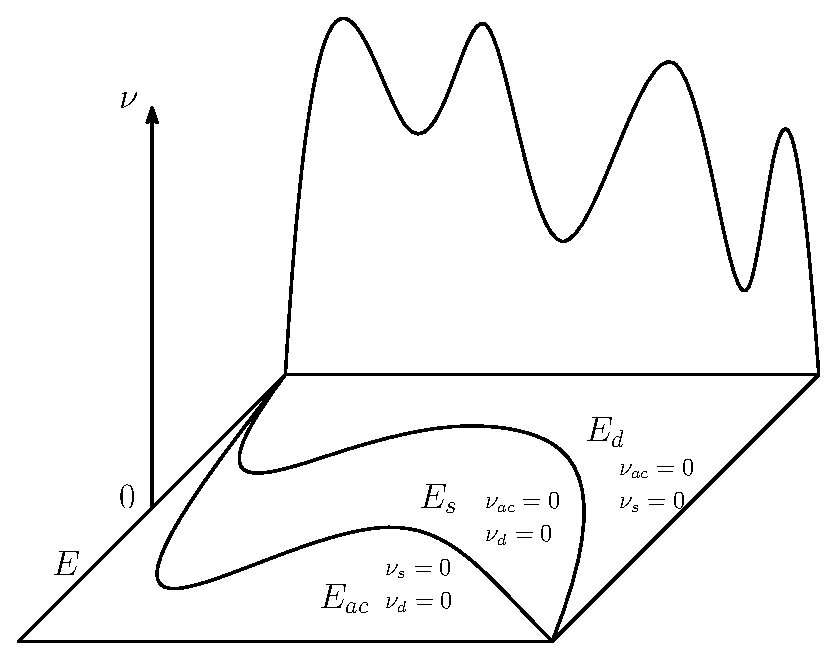
\includegraphics[width=0.7\linewidth]{../notes/img/degiorgi2.eps}
        \end{figure}
    \end{frame}

    \begin{frame}
        \frametitle{Signed Measures}

        \begin{definition} \label{def:signed_measures}
            A function \(\lambda\colon \mathfrak{M} \to [-\infty, \infty]\) is called a \emph{signed measure}, if:
            \begin{enumerate}[label=(\roman*)]
                \item \(\lambda(\emptyset) = 0\)
                \item \(|\{-\infty, \infty\} \cap \text{im}(\lambda)| \leq 1\)
                \item For any mutually disjoint family \(\{E_n \subseteq \mathfrak{M}\}_{n \in \mathbb{N}_{\geq 1}}\), we have \(\lambda\left(\bigcup_{n=1}^\infty E_n\right) = \sum_{n=1}^\infty \lambda(E_n)\).
            \end{enumerate}
        \end{definition}

        \pause

        \begin{lemma} \label{lem:limit_characterization_of_signed_measures}
            A set function \(\lambda\colon \mathfrak{M} \to [-\infty, \infty]\) is a signed measure, iff it satisfies the following:
            \begin{enumerate}[label=(\roman*)]
                \item \(|\{-\infty, \infty\} \cap \text{im}(\lambda)| \leq 1\)
                \item \(\lambda(E \cup F) = \lambda(E) + \lambda(F)\) for disjoint \(E, F \in \mathfrak{M}\).
                \item For any increasing sequence \(\{E_n \subseteq \mathfrak{M}\}_{n \in \mathbb{N}_{\geq 1}}\), we have \(\lambda\left(\bigcup_{n=1}^\infty E_n\right) = \lim_{n \to \infty} \lambda(E_n)\).
            \end{enumerate}
        \end{lemma}
    \end{frame}

    \begin{frame}
        \frametitle{Positive Sets}

        \begin{definition}
            A set \(E \in \mathfrak{M}\) is called \emph{positive}, if \(\lambda(F) \geq 0\), and resp. \emph{negative}, if \(\lambda(F) \leq 0\), for all \(\mathfrak{M} \ni F \subseteq E\).
        \end{definition}

        \pause

        \begin{lemma} \label{lem:existence_of_positive_subset}
            Let \(E \in \mathfrak{M}\) with \(\lambda(E) \in (0, \infty)\). Then there exists a positive \(\mathfrak{M} \ni F \subseteq E\).
        \end{lemma}
    \end{frame}

    \begin{frame}
        \frametitle{Hahn Decomposition}

        \begin{theorem}[Hahn Decomposition Theorem] \label{thm:hahn_decomposition}
            Any measurable space \((X, \mathfrak{M})\) can be decomposed as \(X = X^+ \cup X^-\), where \(X^+ \subseteq X\) is positive and \(X^- \subseteq X\) is negative.
        \end{theorem}

        \pause

        \begin{figure}[!hbtp]
            \centering
            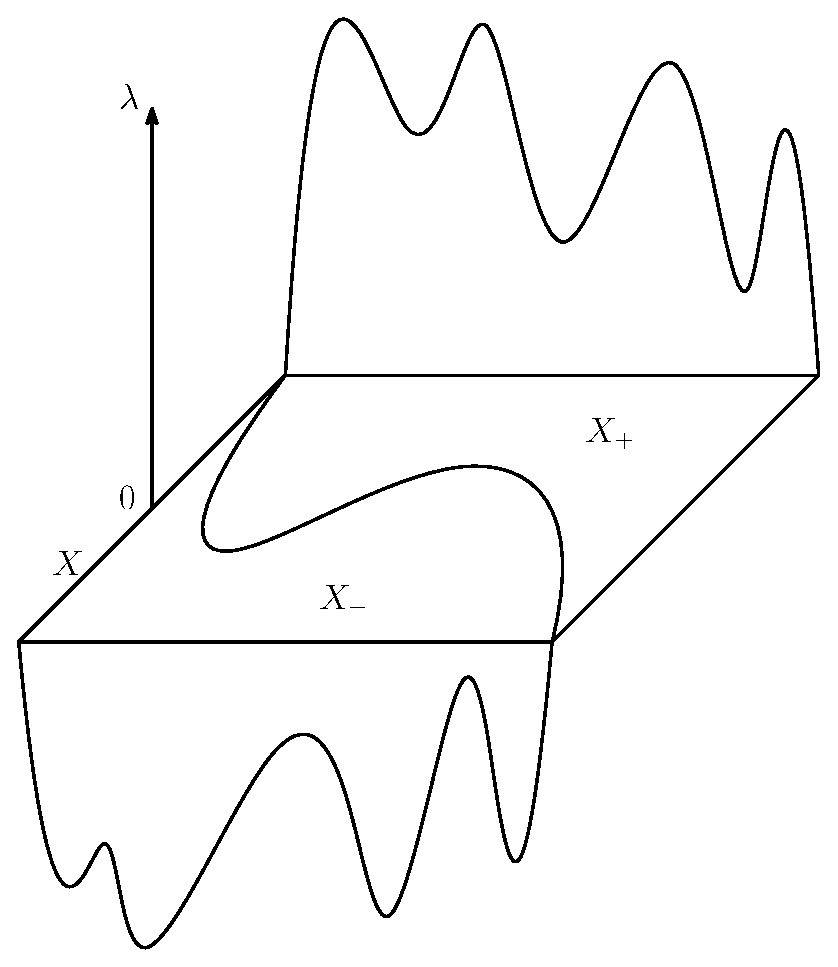
\includegraphics[width=0.4\linewidth]{../notes/img/hahn.eps}
        \end{figure}
    \end{frame}

    \begin{frame}
        \frametitle{Jordan Decomposition}

        \begin{theorem}[Jordan Decomposition Theorem] \label{thm:jordan_decomposition}
            There exists a unique pair \((\lambda^+, \lambda^-)\) of measures with \(\lambda^+ \perp \lambda^-\), one being finite and \(\lambda = \lambda^+ - \lambda^-\).
        \end{theorem}

        \pause

        \(\leadsto\) Lebesgue integral definition.
    \end{frame}

    \begin{frame}
        \frametitle{Signed Lebesgue Decomposition}

        \enquote{Culmination Theorem}.

        \begin{theorem}[Signed Lebesgue Decomposition Theorem]
            Let \(\lambda\colon \mathfrak{M} \to [-\infty, \infty]\) be a signed measure and \(\mu\colon \mathfrak{M} \to [0, \infty]\) be a \(\sigma\)-finite measure.
            \begin{enumerate}[label=(\roman*), wide]
                \item \label{thm:lebesgue_decomposition_thm_1} There are signed measures \(\lambda_{ac}, \lambda_s\colon X \to [-\infty, \infty]\) and a measurable function \(u\colon X \to [-\infty, \infty]\) with
                \begin{align}
                    \lambda = \lambda_{ac} + \lambda_s,
                \end{align}
                \(\lambda_{ac} \ll \mu\) and
                \begin{align}
                    \lambda_{ac}(\cdot) = \int_{\cdot} u \, d\mu.
                \end{align}
                \item \label{thm:lebesgue_decomposition_thm_2} If \(\lambda\) is \(\sigma\)-finite, then \(\lambda_s \perp \mu\) and the decomposition is unique.
            \end{enumerate}
        \end{theorem}
    \end{frame}

    \begin{frame}
        \frametitle{Summary}

        \begin{minipage}{\linewidth}
            \centering
            \begin{tabular}{C{4cm}|C{3cm}}
                Decomposition & Summary \\\hline
                Hewitt-Yosida \cite[pp. 8-9]{Fonseca} & \(\mu = \mu_p + \mu_c\)\\
                Atomic \cite[pp. 13-16]{Fonseca} & \(\mu = \mu_1 + \mu_2\)\\
                Lebesgue & \(\nu = \nu_{ac} + \nu_s\)\\
                De Giorgi & \(\nu = \nu_{ac} + \nu_s + \nu_d\)\\
                Hahn & \(X = X^+ \cup X^-\)\\
                Jordan & \(\lambda = \lambda^+ - \lambda^-\)\\
                Signed Lebesgue & \(\lambda = \lambda_{ac} + \lambda_s\)
            \end{tabular}
        \end{minipage}
    \end{frame}

    \begin{frame}
        \frametitle{References}

        The main source of this presentation is \cite{Fonseca}, additionally the books \cite{Axler} and \cite{Elstrodt} were used.

        \printbibliography{}
    \end{frame}
\end{document}
